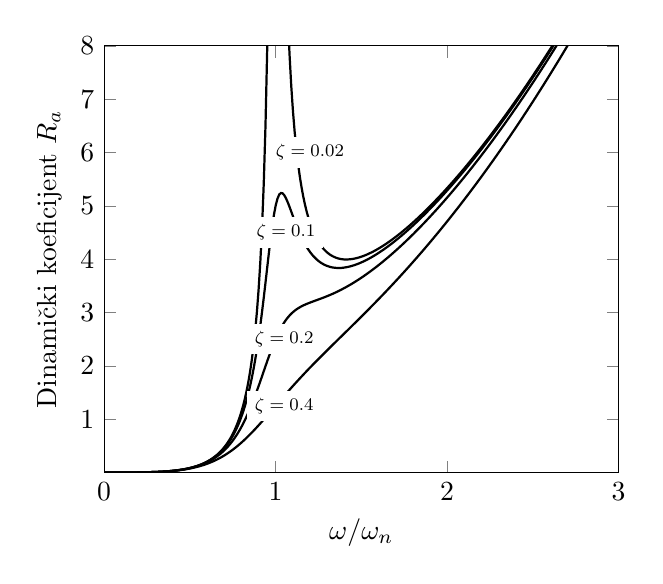
\begin{tikzpicture}
    \begin{axis} [
        height=7cm,
        ylabel = Dinamički koeficijent $R_a$,
        xlabel = $\omega/\omega_n$,
        xmin = 0, xmax = 3,
        ymin = 0, ymax = 8,
        xtick = {0, 1, 2, 3},
        ytick = {1, 2, 3, 4, 5, 6, 7, 8},
     ]

    \foreach \i in {0.4, 0.2, 0.1, 0.02}
        {
            \addplot [
                domain=0:10,
                samples=1000,
                color=black,
                thick,
            ]{x^4/((1-x^2)^2+(2*\i*x)^2)^0.5};
        }
   \pgfplotsinvokeforeach{0.4,0.2}
        {
            \node[rectangle,fill=white,scale=0.8] at 
                (1.05,{1/(2*#1)}) {\footnotesize{$\zeta=#1$}};
        }
    \node[rectangle,fill=white,scale=0.8] at 
        (1.06,4.5) {\footnotesize{$\zeta=0.1$}};

    \node[rectangle,fill=white,scale=0.8] at 
        (1.2,6) {\footnotesize{$\zeta=0.02$}};
    \end{axis}

\end{tikzpicture}
